\documentclass[
11pt, % The default document font size, options: 10pt, 11pt, 12pt
%codirector, % Uncomment to add a codirector to the title page
]{charter} 




% El títulos de la memoria, se usa en la carátula y se puede usar el cualquier lugar del documento con el comando \ttitle
\titulo{Sistema de monitoreo para planta de acopio de cereales} 

% Nombre del posgrado, se usa en la carátula y se puede usar el cualquier lugar del documento con el comando \degreename
%\posgrado{Carrera de Especialización en Sistemas Embebidos} 
\posgrado{Carrera de Especialización en Internet de las Cosas} 
%\posgrado{Carrera de Especialización en Intelegencia Artificial}
%\posgrado{Maestría en Sistemas Embebidos} 
%\posgrado{Maestría en Internet de las cosas}

% Tu nombre, se puede usar el cualquier lugar del documento con el comando \authorname
\autor{Ing. Lucas Eduardo Olmedo} 

% El nombre del director y co-director, se puede usar el cualquier lugar del documento con el comando \supname y \cosupname y \pertesupname y \pertecosupname
\director{Marcelo Castello}
\pertenenciaDirector{pertenencia} 
% FIXME:NO IMPLEMENTADO EL CODIRECTOR ni su pertenencia
\codirector{John Doe} % para que aparezca en la portada se debe descomentar la opción codirector en el documentclass
\pertenenciaCoDirector{FIUBA}

% Nombre del cliente, quien va a aprobar los resultados del proyecto, se puede usar con el comando \clientename y \empclientename
\cliente{Tribunal Jurado trabajo final CEIoT}
\empresaCliente{FIUBA}

% Nombre y pertenencia de los jurados, se pueden usar el cualquier lugar del documento con el comando \jurunoname, \jurdosname y \jurtresname y \perteunoname, \pertedosname y \pertetresname.
\juradoUno{Nombre y Apellido (1)}
\pertenenciaJurUno{pertenencia (1)} 
\juradoDos{Nombre y Apellido (2)}
\pertenenciaJurDos{pertenencia (2)}
\juradoTres{Nombre y Apellido (3)}
\pertenenciaJurTres{pertenencia (3)}
 
\fechaINICIO{28 de febrero de 2023}		%Fecha de inicio de la cursada de GdP \fechaInicioName
\fechaFINALPlan{24 de abril de 2023} 	%Fecha de final de cursada de GdP
\fechaFINALTrabajo{15 de febrero de 2024}	%Fecha de defensa pública del trabajo final


\begin{document}

\maketitle
\thispagestyle{empty}
\pagebreak


\thispagestyle{empty}
{\setlength{\parskip}{0pt}
\tableofcontents{}
}
\pagebreak


\section*{Registros de cambios}
\label{sec:registro}


\begin{table}[ht]
\label{tab:registro}
\centering
\begin{tabularx}{\linewidth}{@{}|c|X|c|@{}}
\hline
\rowcolor[HTML]{C0C0C0} 
Revisión & \multicolumn{1}{c|}{\cellcolor[HTML]{C0C0C0}Detalles de los cambios realizados} & Fecha      \\ \hline
0      & Creación del documento                                 &\fechaInicioName \\ \hline
1      & Se completa hasta el punto 5 inclusive                 & 12 de marzo de 2023 \\ \hline
%2      & Se completa hasta el punto 7 inclusive
%		  Se puede agregar algo más \newline
%		  En distintas líneas \newline
%		  Así                                                    & dd/mm/aaaa \\ \hline
%3      & Se completa hasta el punto 11 inclusive                & dd/mm/aaaa \\ \hline
%4      & Se completa el plan	                                 & dd/mm/aaaa \\ \hline
\end{tabularx}
\end{table}

\pagebreak



\section*{Acta de constitución del proyecto}
\label{sec:acta}

\begin{flushright}
Buenos Aires, \fechaInicioName
\end{flushright}

\vspace{2cm}

Por medio de la presente se acuerda con el \authorname\hspace{1px} que su Trabajo Final de la \degreename\hspace{1px} se titulará ``\ttitle'', consistirá esencialmente en la implementación de un prototipo de un sistema para monitorear plantas de acopio de cereales, y tendrá un presupuesto preliminar estimado de 600 h de trabajo y \textcolor{red}{\$XXX}, con fecha de inicio \fechaInicioName\hspace{1px} y fecha de presentación pública \fechaFinalName.

Se adjunta a esta acta la planificación inicial.

\vfill

% Esta parte se construye sola con la información que hayan cargado en el preámbulo del documento y no debe modificarla
\begin{table}[ht]
\centering
\begin{tabular}{ccc}
\begin{tabular}[c]{@{}c@{}}Dr. Ing. Ariel Lutenberg \\ Director posgrado FIUBA\end{tabular} & \hspace{2cm} & \begin{tabular}[c]{@{}c@{}}\clientename \\ \empclientename \end{tabular} \vspace{2.5cm} \\ 
\multicolumn{3}{c}{\begin{tabular}[c]{@{}c@{}} \supname \\ Director del Trabajo Final\end{tabular}} \vspace{2.5cm} \\
%\begin{tabular}[c]{@{}c@{}}\jurunoname \\ Jurado del Trabajo Final\end{tabular}     &  & \begin{tabular}[c]{@{}c@{}}\jurdosname\\ Jurado del Trabajo Final\end{tabular}  \vspace{2.5cm}  \\
%\multicolumn{3}{c}{\begin{tabular}[c]{@{}c@{}} \jurtresname\\ Jurado del Trabajo Final\end{tabular}} \vspace{.5cm}                                                                     
\end{tabular}
\end{table}




\section{1. Descripción técnica-conceptual del proyecto a realizar}
\label{sec:descripcion}

El presente proyecto es un emprendimiento personal dirigido a solucionar un problema detectado en algunas plantas de acopio de cereales. Una empresa  o cooperativa dedicada al almacenamiento de granos tiene uno o más depósitos distribuidos y para controlar el estado de almacenamiento de sus productos necesita enviar operarios a las diferentes plantas. Dada esta situación, se plantea implementar un sistema de monitoreo IoT para optimizar tiempos y costos. 

Una planta de acopio se encarga de recepcionar diferentes diferentes tipos de granos, analizarlos, secarlos y almacenarlos. Para ello, dispone de silos equipados con sistemas de ventilación y control de termométricos, con el objetivo de minimizar las pérdidas de granos tanto en forma cuantitativa como cualitativa durante la etapa de almacenamiento. 

Una empresa que brinde servicio de almacenamiento puede tener varias plantas de acopio distribuidas en diferentes ciudades o zonas rurales. El objetivo del sistema IoT a desarrollar es simplificar la tarea de administración que puede tener una empresa o cooperativa. Se propone instalar nodos y sensores identificando cada silo, monitorizar el estado del cereal almacenado y centralizar esta información en la nube. Con este sistema será posible trazar el estado de almacenamiento del cereal, disminuir las tareas manuales del personal en cada planta y administrar más de una planta desde una sola oficina. 

Si bien en el mercado se encuentran algunas ofertas de sistemas IoT para silos, se plantea diseñar una solución a medida mediante la reutilización de instalaciones existentes y brindando así la posibilidad de reciclar sensores. La propuesta es instalar un nodo por cada silo, este debe obtener datos de sensores para luego transmitirlos hacia la nube. 

La solución propuesta se compone de las siguientes partes: 
\begin{itemize}
	\item Obtención de datos desde sensores. 
	\item Adaptar y transmitir datos a la nube.
	\item Procesamiento y persistencia de datos.
	\item Presentación de datos y alarmas. 
\end{itemize}

En la Figura \ref{fig:diagBloques} se presenta el diagrama en bloques del sistema. Se observa que cada planta de acopio esta compuesta de silos, cada uno de estos posee un nodo con uno o mas sensores. Los nodos transmiten los datos a la nube, los cuales serán almacenados en un servidor de bases de datos y presentados en un \textit{dashboard} o aplicación en las oficinas de la empresa o cooperativa.

\begin{figure}[htpb]
\centering 
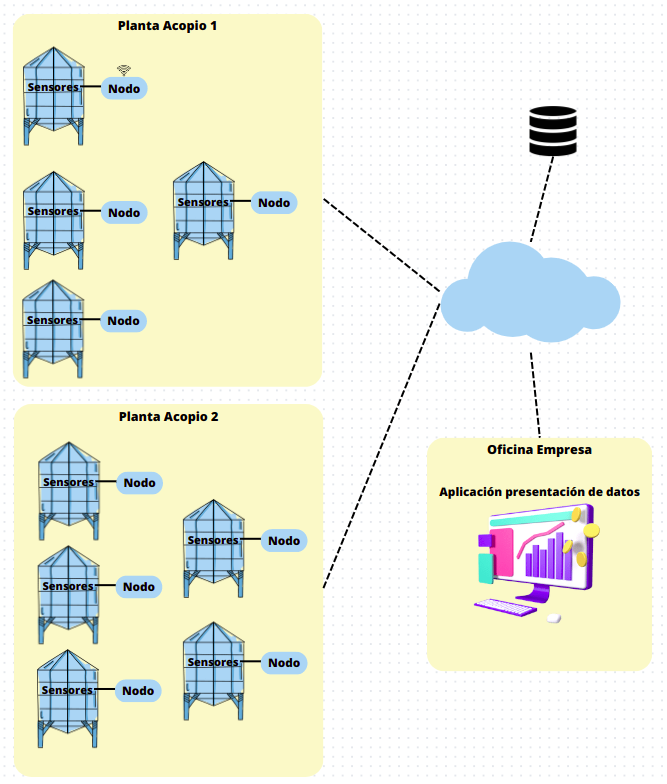
\includegraphics[width=.9\textwidth]{./Figuras/PlantaAcopio.png}
\caption{Diagrama en bloques del sistema}
\label{fig:diagBloques}
\end{figure}

\vspace{25px}

\section{2. Identificación y análisis de los interesados}
\label{sec:interesados}

\begin{table}[ht]
%\caption{Identificación de los interesados}
%\label{tab:interesados}
\begin{tabularx}{\linewidth}{@{}|l|X|X|l|@{}}
\hline
\rowcolor[HTML]{C0C0C0} 
Rol           & Nombre y Apellido    & Organización 	& Puesto 	\\ \hline
%Auspiciante   &                     &              	&        	\\ \hline
Cliente       & \clientename         &\empclientename	&--       	\\ \hline
%Impulsor      &                     &              	&        	\\ \hline
Responsable   & \authorname          & FIUBA        	& Alumno 	\\ \hline
%Colaboradores &                     &              	&        	\\ \hline
Orientador    & \supname	         & \pertesupname 	& Director Trabajo final \\ \hline
%Equipo        & miembro1 \newline 
%				miembro2             &              	&        	\\ \hline
%Opositores    &--                   &Empresas de la competencia   	&--        	\\ \hline
Usuario final &Empleados Oficina     & Empresa de Acopio   	& Operador / Administrador        	\\ \hline
\end{tabularx}
\end{table}

\begin{itemize}
	\item Cliente: es el jurado del trabajo final de la especialización de IoT. Todavía a definir. 
\end{itemize}



\section{3. Propósito del proyecto}
\label{sec:proposito}

El propósito de este proyecto es implementar un sistema de monitoreo para el almacenamiento de cereales, con el objetivo de conservar en condiciones óptimas los granos almacenados. El sistema deberá diseñarse e implementarse utilizando los conocimientos adquiridos durante el cursado de la CEIoT y con miras a su implementación en campo a futuro. 

\section{4. Alcance del proyecto}
\label{sec:alcance}

El alcance del proyecto incluye:

\begin{itemize}
 \item Un prototipo funcional. 
 \item Al menos un nodo instalado en un silo que simule datos obtenidos y transmita los mismos a la nube. 
 \item Selección del protocolo para transmisión de datos. 
 \item Desarrollo de \textit{backend} del sistema que procese y almacene los datos recibidos.
 \item Presentación de datos en una aplicación.
\end{itemize}

El presente proyecto no incluye: 

\begin{itemize}
 \item La puesta en marcha del producto en las instalaciones de una planta de almacenamiento.
 \item La lectura de datos en sensores reales desde los nodos.
\end{itemize}




\section{5. Supuestos del proyecto}
\label{sec:supuestos}

Para el desarrollo del presente proyecto se supone que: 

\begin{itemize}
	\item Se implementa un prototipo para el trabajo final de CEIoT, pero el proyecto se continuara. 
	\item Las plantas de acopio disponen de una conexión a internet. 
	\item Se dispone de la colaboración de personas idóneas en el almacenamiento de cereales.
	\item Se dispone continuidad de los recursos humanos necesarios durante el desarrollo del proyecto. 
	\item Se contará con los recursos económicos necesarios para la realización del proyecto. 
	\item Se cuenta con el \textit{hardware} necesario para implementar al menos un prototipo.
	\item El cliente acepta que las mediciones de temperatura y cantidad de cereal en un silo sean simuladas. 
\end{itemize}


\section{6. Requerimientos}
\label{sec:requerimientos}

\begin{enumerate}
	\item Requerimientos funcionales
		\begin{enumerate}
			\item El sistema deberá monitorizar silos de diferentes plantas de acopio.
			\item El sistema deberá obtener la temperatura de los silos y transmitirla cada 10 minutos.
			\item El sistema deberá obtener la cantidad en kg de cereal almacenado en un silo y transmitirlo cada 15 minutos.
			\item El sistema deberá mostrar la capacidad máxima de almacenamiento de cada silo y el tipo de cereal almacenado.
			\item El sistema deberá transmitir los datos de forma segura desde los nodos sensores a un servidor. 
			\item El sistema deberá contar con una interfaz gráfica donde se presenten los datos obtenidos.
			\item La interfaz gráfica se debe poder acceder por los usuarios de la empresa en diferentes computadoras.
			\item El sistema deberá generar alertas a los usuarios cuando un silo supere una determinada temperatura. 
			\item El sistema deberá almacenar el historial de mediciones por cada silo en una base de datos. 
			\item El sistema deberá mostrar en tiempo real las mediciones de un silo. 
			\item El sistema deberá mostrar el historial de mediciones de un silo.
			\item El sistema deberá mostrar todos los silos de una planta indicando si las mediciones de temperatura de un silo están fuera de un rango establecido. 
		\end{enumerate}
	\item Requerimientos no funcionales
		\begin{enumerate}
			\item El sistema deberá ser escalable, permitiendo agregar mas plantas de acopio dentro de una empresa, mas silos en una planta y mas sensores en un silo.  
			\item El sistema debe estar protegido contra el acceso no autorizado.
			\item El sistema debe tener una interfaz intuitiva y documentación clara para facilitar su uso por parte del usuario.
		\end{enumerate}	
	\item Requerimientos de documentación
		\begin{enumerate}
			\item Se debe generar un documento de planificación del proyecto.
			\item Se debe generar un manual de uso.
			\item Se debe generar un manual de instalación.
			\item Se debe generar una memoria técnica con la documentación de ingeniería detallada.			
		\end{enumerate}
\end{enumerate}

\section{7. Historias de usuarios (\textit{Product backlog})}
\label{sec:backlog}

\textit{Story points}: Se utilizarán 1, 2, 3, 5, 8 y 13 para la estimación de las historias de usuario, según la
serie de Fibonacci.
Los \textit{story points} se asignan a una tarea o historia de usuario en función de la complejidad que representa para el equipo de proyecto. La asignación de \textit{story points} se basa en una evaluación en equipo de varios factores como: esfuerzo requerido, dificultad, complejidad e incertidumbre.

\begin{itemize}
\item Como cliente quiero visualizar todas las plantas de acopio de la empresa en una sola aplicación para tener el control desde una o varias oficinas. (\textit{Story points}: 3)

\item Como cliente quiero ver la temperatura de un silo en tiempo real en una aplicación para controlar el estado de conservación del cereal a distancia. (\textit{Story points}: 5)

\item Como cliente quiero saber la cantidad de cereal almacenado en un silo para poder decidir si es posible almacenar mas cereal en este.  (\textit{Story points}: 5)

\item Como cliente quiero tener información de la capacidad restante de almacenamiento de un silo y el tipo de cereal para poder realizar logística sin necesidad de ir a la planta. (\textit{Story points}: 2)

\item Como cliente quiero visualizar una alarma cuando un silo supere una temperatura determinada, indicando la planta y silo correspondiente para poder tomar acciones preventivas y mantener el cereal en optimo estado. (\textit{Story points}: 2)

\item Como cliente quiero poder visualizar el historial de mediciones de un silo para controlar el estado del almacenamiento del cereal. (\textit{Story points}: 8)

\item Como cliente quiero poder acceder a la aplicación desde distintas computadoras para poder monitorizar las plantas de acpopio desde diferentes oficinas. (\textit{Story points}: 3)

\item Como gerente de la empresa quiero que el sistema pida usuario y contraseña al ingresar para que solo puedan acceder personas autorizadas. (\textit{Story points}: 13)
\end{itemize}

\section{8. Entregables principales del proyecto}
\label{sec:entregables}

\begin{itemize}
	\item Manual de uso.
	\item Manual de instalación.
	\item Prototipo funcional.
	\item Diagrama esquemático de la solución.
	\item Informe final.
	\item Presentación.
\end{itemize}

\section{9. Desglose del trabajo en tareas}
\label{sec:wbs}

\begin{enumerate}
\item Planificación y definición del proyecto (55 h)
	\begin{enumerate}
	\item Investigación preliminar (25 h)
	\item Relevar requerimientos(15 h)
	\item Documentar planificación del proyecto (15 h)
	\end{enumerate}
\item Protocolo de comunicación (24 h)
	\begin{enumerate}
	\item Investigación y elección de protocolo de comunicación (24 h)
	\end{enumerate}
\item Análisis y Diseño del modelo de datos (44 h)
	\begin{enumerate}
	\item Elección de tecnología (4 h)
	\item Diseño del modelo de datos (20 h)
	\item Implementación base de datos y carga inicial de datos (20 h)
	\end{enumerate}
\item Diseño e implementación del nodo y mediciones simuladas (76 h)
	\begin{enumerate}
	\item Elección del \textit{hardware} (4 h)
	\item Simulación adquisición de temperatura (20 h)
	\item Simulación nivel de llenado silo en kg (16 h)
	\item Transmisión de datos simulados (20 h)
	\item Pruebas de funcionalidad del nodo (16 h)
	\end{enumerate}	
\item Planificación y desarrollo del \textit{backend} (64 h)
	\begin{enumerate}
	\item Especificación de los requerimientos del \textit{backend} (8 h)
	\item Desarrollo del \textit{backend} (40 h)
	\item Pruebas de funcionalidad del \textit{backend} (16 h)
	\end{enumerate}
\item Planificación y desarrollo del \textit{frontend} (80 h)
	\begin{enumerate}
	\item Especificación de los requerimientos del \textit{frontend} (8 h)
	\item Desarrollo del \textit{frontend} (40 h)
	\item Desarrollo de la comunicación con la base de datos (16 h)
	\item Pruebas de funcionalidad del \textit{frontend} (16 h) 
	\end{enumerate}
\item Diseño e implementación de un sistema de acceso al software (68 h)
	\begin{enumerate}
	\item Especificación de requerimientos de acceso (12 h)
	\item Desarrollo del sistema de acceso (32 h)
	\item Pruebas del sistema de acceso (24 h) 
	\end{enumerate}		
\item Pruebas finales (63 h)
	\begin{enumerate}
	\item Planificación de las pruebas (12 h) 
	\item Generación del ambiente de pruebas (35 h)
	\item Ejecución de las pruebas (16 h)
	\end{enumerate}
\item Documentación (60 h)
	\begin{enumerate}
	\item Generación del manual de instalación (28 h)
	\item Generación del manual del usuario (32 h)
	\end{enumerate}
\item Actividades de cierre (80 h)
	\begin{enumerate}
	\item Generación de la memoria final (48 h)
	\item Generación de video de uso (16 h)
	\item Elaboración de la presentación (16 h) 
	\end{enumerate}
\end{enumerate}

Cantidad total de horas: (614 h).

\section{10. Diagrama de Activity On Node}
\label{sec:AoN}

La unidad de tiempo del diagrama AoN que se muestra en la Figura \ref{fig:AoN} esta expresada en horas.

\begin{figure}[htpb]
\centering 
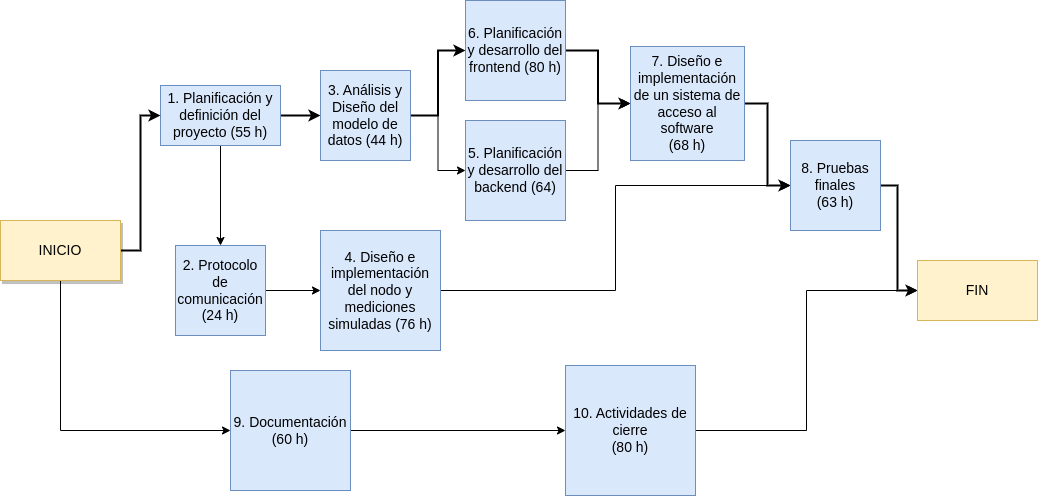
\includegraphics[width=1\textwidth]{./Figuras/DiagramaActivityONNode.png}
\caption{Diagrama de \textit{Activity on Node}.}
\label{fig:AoN}
\end{figure}

\begin{itemize}
	\item El camino critico es de 310 h y esta compuesto por la secuencia de tareas 1-3-6-7-8.
	\item El camino semi critico es de 294 h y esta compuesto por la secuencia de tareas 1-3-5-7-8.
\end{itemize}

\section{11. Diagrama de Gantt}
\label{sec:gantt}



En la figura \ref{fig:TareasGant}, se muestra el desglose de tareas del diagrama de gant.

En las figuras \ref{fig:diagGantt1} y \ref{fig:diagGantt2} se observa el diagrama de gantt. Se considero un recurso trabajando los días martes y jueves 4h por día y los sábados 8h. 

\begin{landscape}
\begin{figure}[htpb]
\centering 
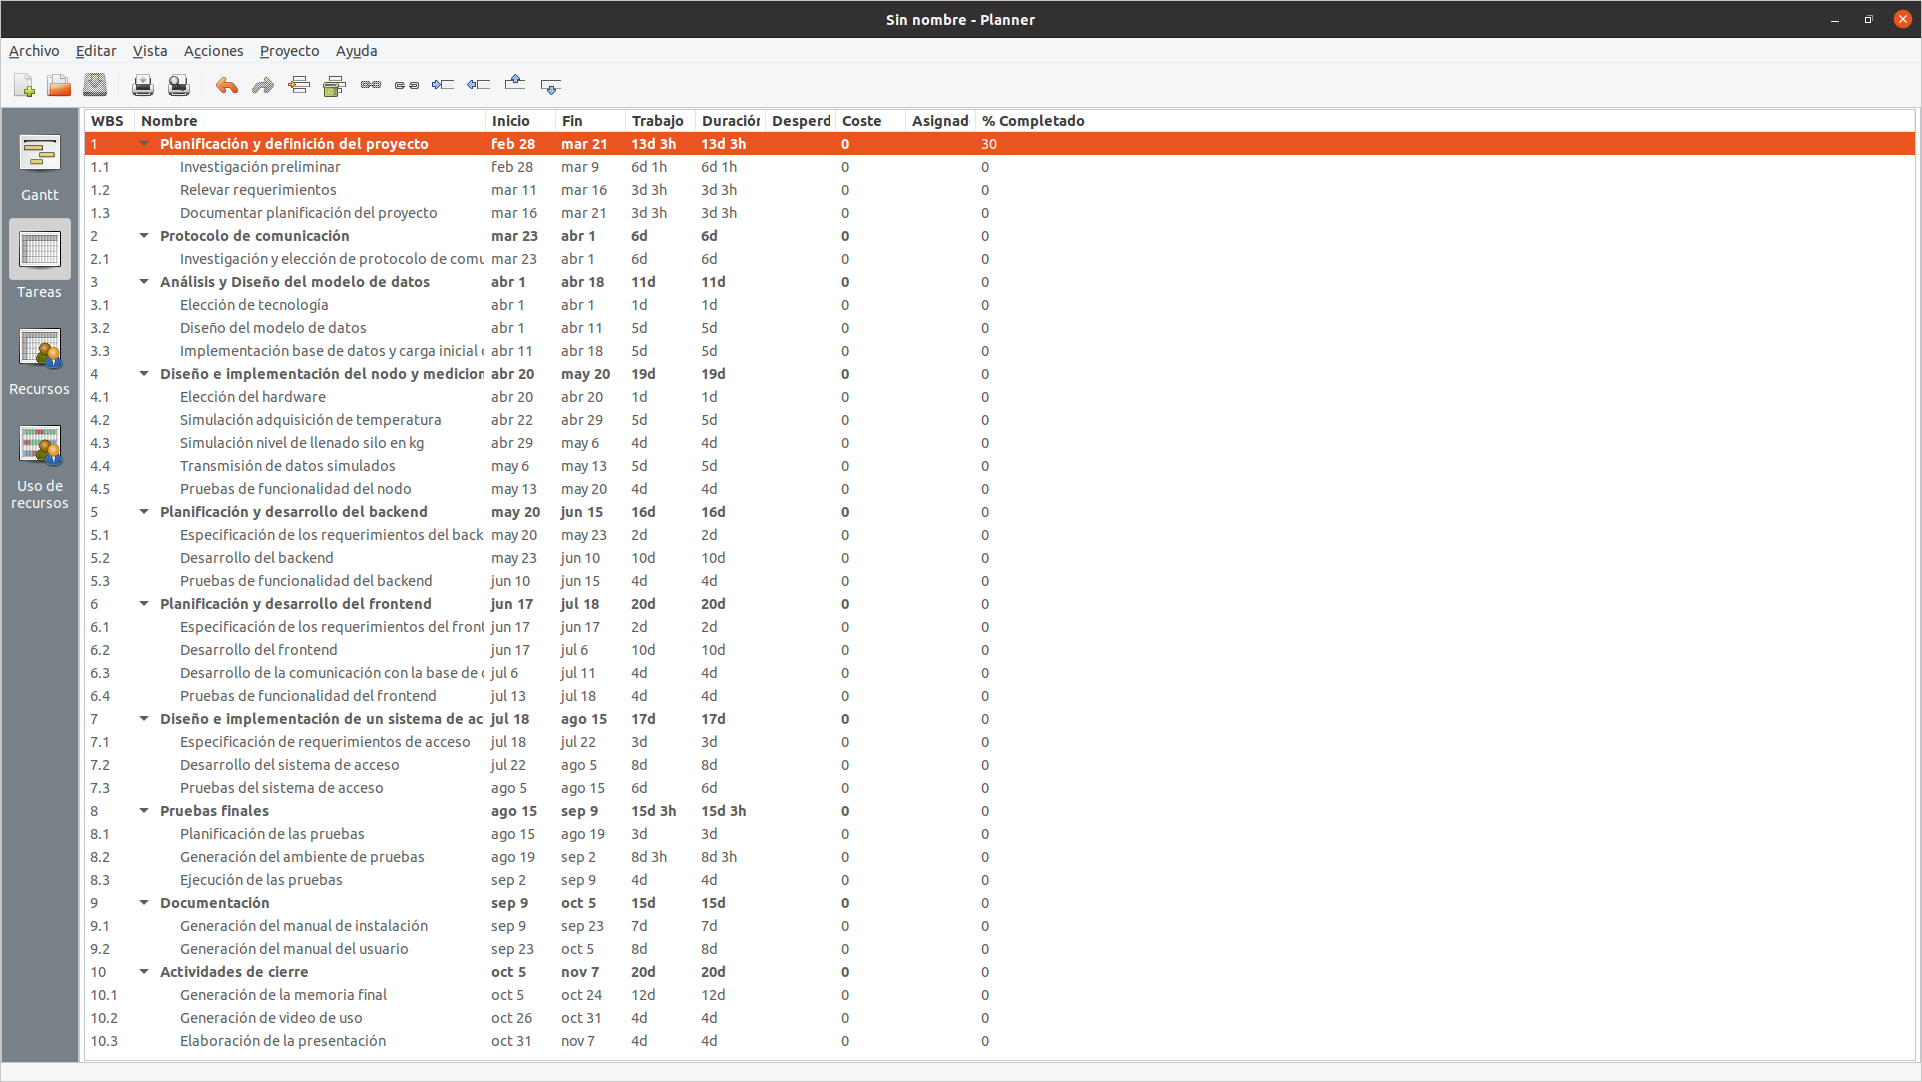
\includegraphics[height=.85\textheight]{./Figuras/TareasGant.png}
\caption{Diagrama de Gantt parte 1}
\label{fig:TareasGant}
\end{figure}
\end{landscape}

\begin{landscape}
\begin{figure}[htpb]
\centering 
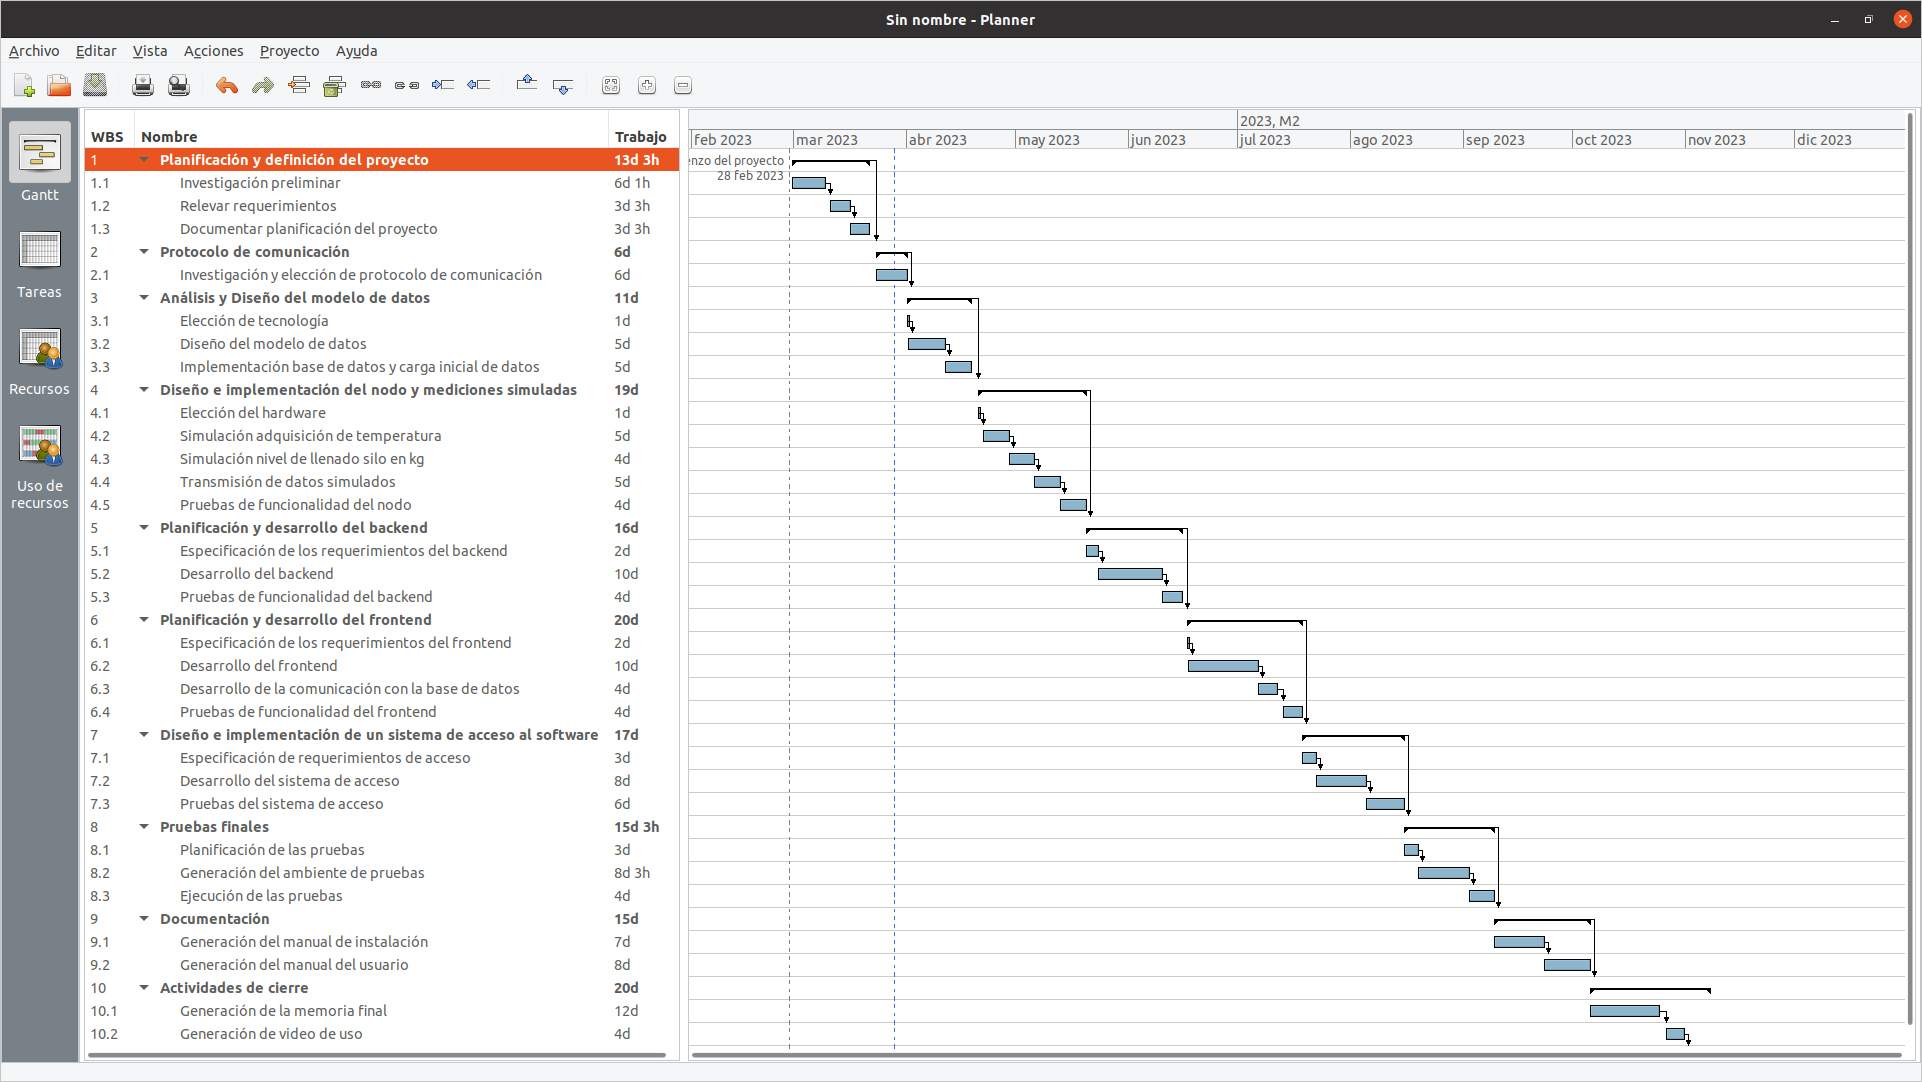
\includegraphics[height=.85\textheight]{./Figuras/DiagramaGant1.png}
\caption{Diagrama de Gantt parte 1}
\label{fig:diagGantt1}
\end{figure}

\end{landscape}

\begin{landscape}
\begin{figure}[htpb]
\centering 
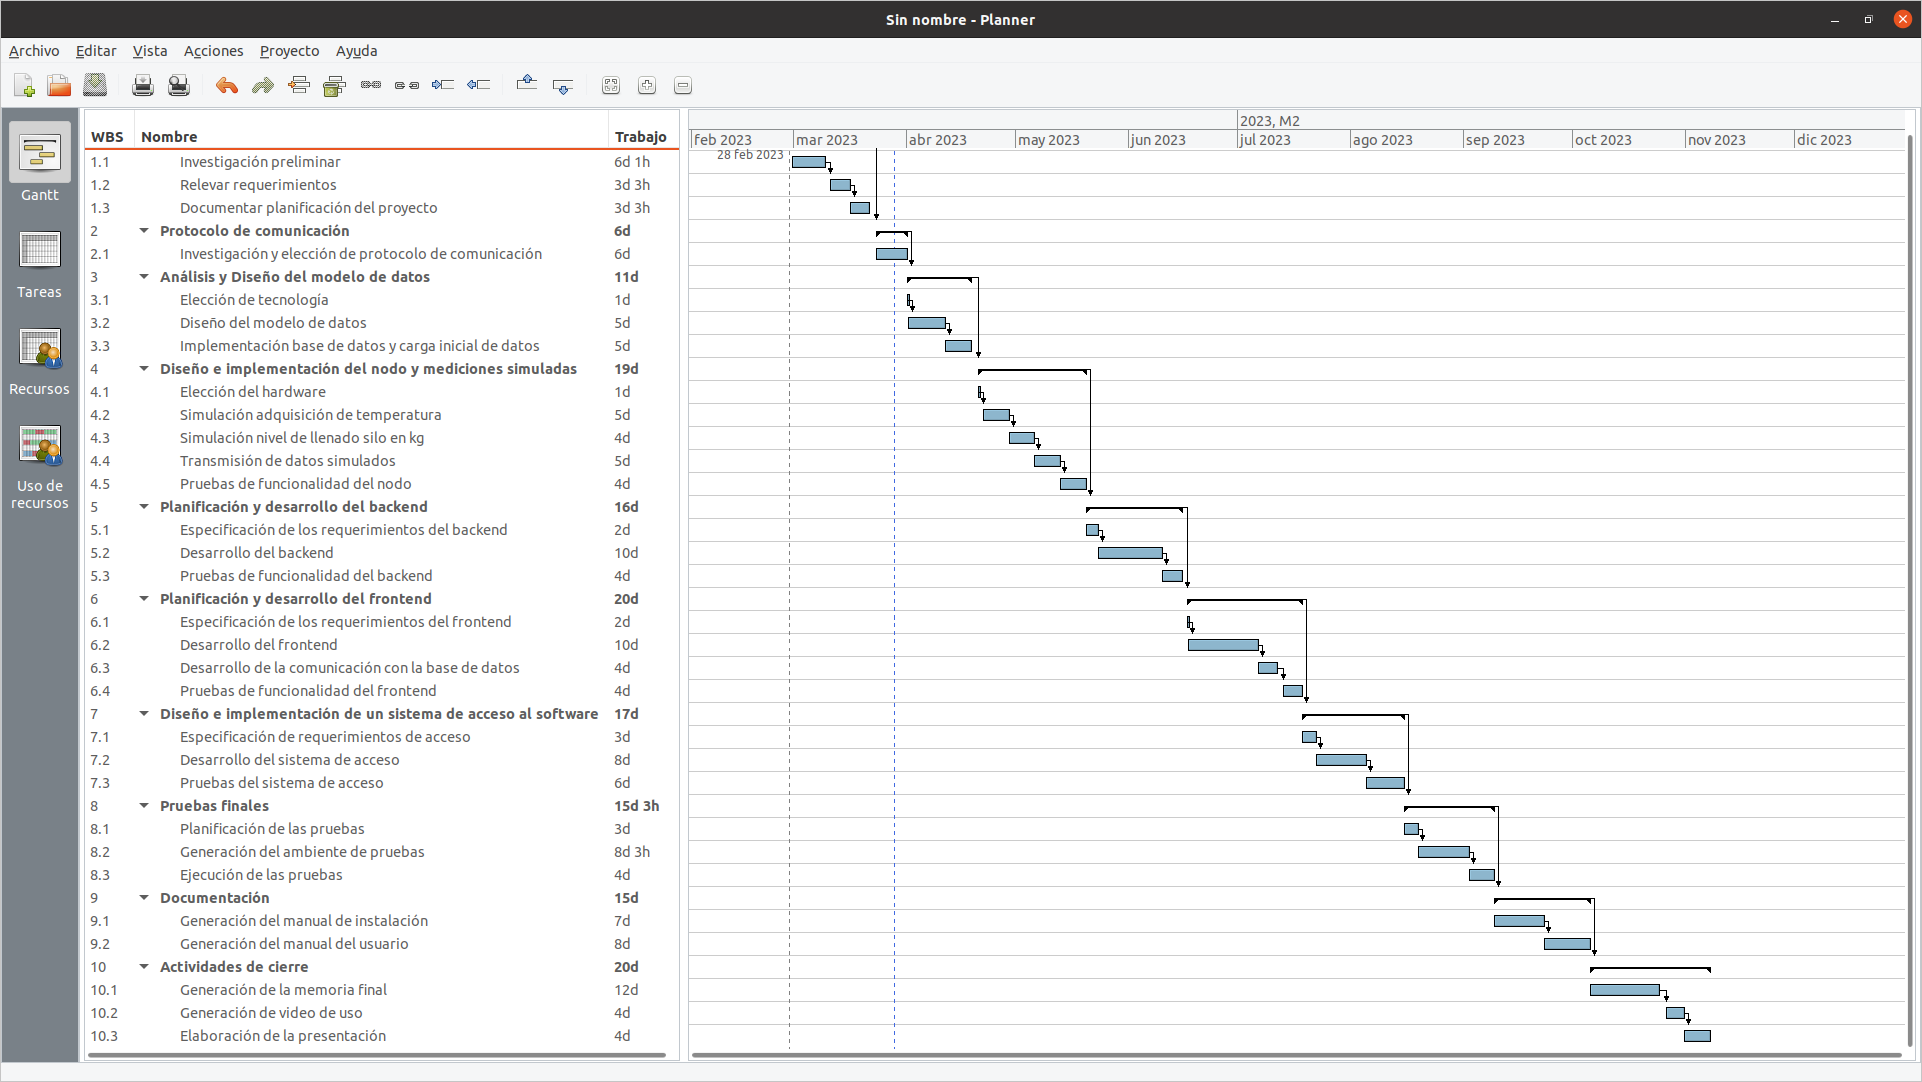
\includegraphics[height=.85\textheight]{./Figuras/DiagramaGant2.png}
\caption{Diagrama de Gantt parte 2}
\label{fig:diagGantt2}
\end{figure}

\end{landscape}


\section{12. Presupuesto detallado del proyecto}
\label{sec:presupuesto}

\begin{table}[htpb]
\centering
\begin{tabularx}{\linewidth}{@{}|X|c|r|r|@{}}
\hline
\rowcolor[HTML]{C0C0C0} 
\multicolumn{4}{|c|}{\cellcolor[HTML]{C0C0C0}COSTOS DIRECTOS} \\ \hline
\rowcolor[HTML]{C0C0C0} 
Descripción &
  \multicolumn{1}{c|}{\cellcolor[HTML]{C0C0C0}Cantidad} &
  \multicolumn{1}{c|}{\cellcolor[HTML]{C0C0C0}Valor unitario} &
  \multicolumn{1}{c|}{\cellcolor[HTML]{C0C0C0}Valor total} \\ \hline
Hardware nodos&
  \multicolumn{1}{c|}{-} &
  \multicolumn{1}{c|}{150000} &
  \multicolumn{1}{c|}{150000} \\ \hline
Horas ingeniería&
  \multicolumn{1}{c|}{614} &
  \multicolumn{1}{c|}{4000} &
  \multicolumn{1}{c|}{2456000} \\ \hline
Servicios cloud&
  \multicolumn{1}{c|}{-} &
  \multicolumn{1}{c|}{200000} &
  \multicolumn{1}{c|}{200000} \\ \hline
  Montaje y pruebas en campo&
  \multicolumn{1}{c|}{-} &
  \multicolumn{1}{c|}{100000} &
  \multicolumn{1}{c|}{100000} \\ \hline
\multicolumn{3}{|c|}{SUBTOTAL} &
  \multicolumn{1}{c|}{2906000} \\ \hline
\rowcolor[HTML]{C0C0C0} 
\multicolumn{4}{|c|}{\cellcolor[HTML]{C0C0C0}COSTOS INDIRECTOS} \\ \hline
%\rowcolor[HTML]{C0C0C0} 
%Descripción &
%  \multicolumn{1}{c|}{\cellcolor[HTML]{C0C0C0}Cantidad} &
%  \multicolumn{1}{c|}{\cellcolor[HTML]{C0C0C0}Valor unitario} &
%  \multicolumn{1}{c|}{\cellcolor[HTML]{C0C0C0}Valor total} \\ \hline
\multicolumn{3}{|c|}{35\% de los costos directos} &
 %  -&
  \multicolumn{1}{c|}{1017100} \\ \hline
\multicolumn{3}{|c|}{SUBTOTAL} &
  \multicolumn{1}{c|}{1017100} \\ \hline
\rowcolor[HTML]{C0C0C0}
\multicolumn{3}{|c|}{TOTAL} &
   \\ \hline
\end{tabularx}%
\end{table}

Consideraciones:
\begin{itemize}
	\item Los costos son estimados ya que en esta instancia del proyecto no esta definido el \textit{hardware} a utilizar 
	\item Los valores están indicados en pesos argentinos, la tasa de cambio actual es de 1 dólar = 213.50 pesos (Banco nación, 27 de marzo de 2023) 
	\item El costo de la hora de ingeniería se obtiene del costo promedio de la hora para un ingeniero de software con varios años de experiencia. 
\end{itemize}


\section{13. Gestión de riesgos}
\label{sec:riesgos}

\begin{consigna}{red}
a) Identificación de los riesgos (al menos cinco) y estimación de sus consecuencias:
 
Riesgo 1: detallar el riesgo (riesgo es algo que si ocurre altera los planes previstos de forma negativa)
\begin{itemize}
	\item Severidad (S): mientras más severo, más alto es el número (usar números del 1 al 10).\\
	Justificar el motivo por el cual se asigna determinado número de severidad (S).
	\item Probabilidad de ocurrencia (O): mientras más probable, más alto es el número (usar del 1 al 10).\\
	Justificar el motivo por el cual se asigna determinado número de (O). 
\end{itemize}   

Riesgo 2:
\begin{itemize}
	\item Severidad (S): 
	\item Ocurrencia (O):
\end{itemize}

Riesgo 3:
\begin{itemize}
	\item Severidad (S): 
	\item Ocurrencia (O):
\end{itemize}


b) Tabla de gestión de riesgos:      (El RPN se calcula como RPN=SxO)

\begin{table}[htpb]
\centering
\begin{tabularx}{\linewidth}{@{}|X|c|c|c|c|c|c|@{}}
\hline
\rowcolor[HTML]{C0C0C0} 
Riesgo & S & O & RPN & S* & O* & RPN* \\ \hline
       &   &   &     &    &    &      \\ \hline
       &   &   &     &    &    &      \\ \hline
       &   &   &     &    &    &      \\ \hline
       &   &   &     &    &    &      \\ \hline
       &   &   &     &    &    &      \\ \hline
\end{tabularx}%
\end{table}

Criterio adoptado: 
Se tomarán medidas de mitigación en los riesgos cuyos números de RPN sean mayores a...

Nota: los valores marcados con (*) en la tabla corresponden luego de haber aplicado la mitigación.

c) Plan de mitigación de los riesgos que originalmente excedían el RPN máximo establecido:
 
Riesgo 1: plan de mitigación (si por el RPN fuera necesario elaborar un plan de mitigación).
  Nueva asignación de S y O, con su respectiva justificación:
  - Severidad (S): mientras más severo, más alto es el número (usar números del 1 al 10).
          Justificar el motivo por el cual se asigna determinado número de severidad (S).
  - Probabilidad de ocurrencia (O): mientras más probable, más alto es el número (usar del 1 al 10).
          Justificar el motivo por el cual se asigna determinado número de (O).

Riesgo 2: plan de mitigación (si por el RPN fuera necesario elaborar un plan de mitigación).
 
Riesgo 3: plan de mitigación (si por el RPN fuera necesario elaborar un plan de mitigación).

\end{consigna}


\section{14. Gestión de la calidad}
\label{sec:calidad}

\begin{consigna}{red}
Para cada uno de los requerimientos del proyecto indique:
\begin{itemize} 
\item Req \#1: copiar acá el requerimiento.

\begin{itemize}
	\item Verificación para confirmar si se cumplió con lo requerido antes de mostrar el sistema al cliente. Detallar 
	\item Validación con el cliente para confirmar que está de acuerdo en que se cumplió con lo requerido. Detallar  
\end{itemize}

\end{itemize}

Tener en cuenta que en este contexto se pueden mencionar simulaciones, cálculos, revisión de hojas de datos, consulta con expertos, mediciones, etc.  Las acciones de verificación suelen considerar al entregable como ``caja blanca'', es decir se conoce en profundidad su funcionamiento interno.  En cambio, las acciones de validación suelen considerar al entregable como ``caja negra'', es decir, que no se conocen los detalles de su funcionamiento interno.

\end{consigna}

\section{15. Procesos de cierre}    
\label{sec:cierre}

\begin{consigna}{red}
Establecer las pautas de trabajo para realizar una reunión final de evaluación del proyecto, tal que contemple las siguientes actividades:

\begin{itemize}
	\item Pautas de trabajo que se seguirán para analizar si se respetó el Plan de Proyecto original:
	 - Indicar quién se ocupará de hacer esto y cuál será el procedimiento a aplicar. 
	\item Identificación de las técnicas y procedimientos útiles e inútiles que se emplearon, y los problemas que surgieron y cómo se solucionaron:
	 - Indicar quién se ocupará de hacer esto y cuál será el procedimiento para dejar registro.
	\item Indicar quién organizará el acto de agradecimiento a todos los interesados, y en especial al equipo de trabajo y colaboradores:
	  - Indicar esto y quién financiará los gastos correspondientes.
\end{itemize}

\end{consigna}


\end{document}
